\documentclass{article}
\usepackage[utf8]{inputenc}
\usepackage{graphicx}


\title{System Programming HW1}
\author{Zafer ALTAY 161044063 }
\date{March 2021}

\begin{document}

\maketitle

\section{Problems and Solutions}
First, I parsed it using getopt to check the inputs received from the terminal.If there are values entered from the terminal, I assigned that value. If no value is entered, I have assigned special values to those variables.Then I checked these values and took action if there was any input.Also I have defined a flag for all values which is 0 if it does not get 1 if it gets input.Using this, I have found the minimum number of arguments or required arguments. If there are errors, I have printed with stderr.

Second,After getting the necessary inputs, I sent to function.This function scans the given path recursively.When I see the matching file using the given inputs, I save it in the 2D character string in filename8yx format.The number 8 here represents the number of spaces. If one file is inside another, this number of spaces increases by 4.Using this number while writing on the screen, we reach the desired path sequence image.The letter y indicates that it matches the searched file. If it doesn't match I used the letter n (filename8nx).I'll explain later what the letter x is.While browsing as Recursion, if the file is a directory, I first added its name to the array and then call the same function again.If not, I added it to array its name and continued to look for the next file.I used the opendir and readdir features of the dirent.h library to look at the file.In the meantime, I continued by checking to see if it meets the desired features for each file.

Third,While I was printing on the screen, I looked for strings with the 2nd letter y from the end in the 2d array first.If I saw the letter y, I parse the part with the number of spaces in that string and got the number of spaces.Then I replace the x at the end of the string with the letter w, which means it will be typed.If this string is in the 2d array, I will save it in a different array,I will explain why I did it.After this process, I immediately look at the next index, if the number of spaces of that index is less than the number of spaces I have last taken, the element of this index is the parent of the previous element.For example, let aaaa8yw and bbbb4nx be at ordered indices. My last whitespace number is 8 and the one I check now is 4, aaaa is child of the bbbb directory.I go through a loop until the last element and when I find the sub-elements I don't forget to add the letter w at the end and save its location in the array.When looking for file items for another element, if I come across an element with the letter w, I don't save it and stop searching because it will be written anyway, I don't need to check it again.Then, when all the searches were finished, when I sorted the array in which it recorded the index numbers in ascending order and wrote the file names that those indices in the 2d char array, I got the correct path directory.

Fourth,I converted the filename check, the given name and the letters of the filename I read while browsing the files to uppercase.Then I compared the letters one by one, if I saw the letter +, I went forward until it was not the same as the previous letter and continued from there.The reason I capitalize the letters is to remove case sensitivity.

Fifth,For permission check, I checked the 9 different permissions of the file and put it into a string. Then I compared it with the string given as input.

Since no extra processing is needed for other benchmarks, I just checked if they are equal.

\section{Pass/Fail}

I did all the search criteria requested in the homework by searching for files in a recursion way, using the ways I mentioned above.

-Wall control does not show any error and  valgrind does not have a memory leak problem.

I reported errors with stderr due to missing or incorrect arguments.

When I got the Ctrl C signal, I cleared the memory and made a notification, then closed the program.

There are things that seem wrong in Valgrind, but the wall does not look wrong.

If there is such an expectation, this is the only thing missing from the homework.If I haven't missed a bug, I've done all that was expected.
\begin{figure}[b]
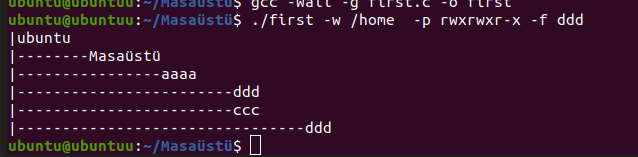
\includegraphics[width=10cm,height=4cm]{ss.png}
\caption{Example Output}
\end{figure}




\end{document}
